\documentclass[12pt,twoside]{article}
\usepackage{mathtools} % for DeclareParedDelimiter
\usepackage{listings}
\usepackage{graphicx} % Required for including images
\newcommand{\reporttitle}{Foundations of Machine Learning}
\newcommand{\reportauthor}{Lionel Ngoupeyou Tondji}
\newcommand{\reporttype}{Assignment: Foundations of Machine Learning (AMMI)}
\newcommand\myeq{\mathrel{\overset{\makebox[0pt]{\mbox{\normalfont\tiny\sffamily iid}}}{=}}}





\begin{document}
% front page

% Last modification: 2016-09-29 (Marc Deisenroth)
\begin{titlepage}
\newcommand{\HRule}{\rule{\linewidth}{0.5mm}} % Defines a new command for the horizontal lines, change thickness here


%----------------------------------------------------------------------------------------
%	LOGO SECTION
%----------------------------------------------------------------------------------------

\begin{center}

\includegraphics[height = 2cm]{qla}\hspace{4mm}

\includegraphics[height=2cm]{aims-rwanda}
\end{center}
 

\begin{center} % Center remainder of the page

%----------------------------------------------------------------------------------------
%	HEADING SECTIONS
%----------------------------------------------------------------------------------------
\textsc{\LARGE \reporttype}\\[1.5cm] 
\textsc{\Large African Institute for Mathematical Sciences}\\[0.5cm] 
\textsc{\large Quantum Leap Africa}\\[0.5cm] 
%----------------------------------------------------------------------------------------
%	TITLE SECTION
%----------------------------------------------------------------------------------------

\HRule \\[0.4cm]
{ \huge \bfseries \reporttitle}\\ % Title of your document
\HRule \\[1.5cm]
\end{center}
%----------------------------------------------------------------------------------------
%	AUTHOR SECTION
%----------------------------------------------------------------------------------------

\begin{minipage}{0.4\hsize}
 \begin{flushleft} \large
 \textit{Author: Lionel Ngoupeyou Tondji}\\
 \end{flushleft}
  \vspace{2cm}
 \makeatletter
 Date: \@date 
\end{minipage}
\vfill % Fill the rest of the page with whitespace



\makeatother

\end{titlepage}




\section*{Density Estimation with Gaussian Mixture Models}

\subsection*{Task 1}

See the python file.

\subsection*{Task 2}

You are given a two-dimensional dataset of about 30 geolocations (latitude/longitude) of birthplaces. Model the data as well as possible. Describe your approach, justify your choices and interpret your results.


First of all we are trying to plot the two-dimensional dataset, to see how they look like.
\begin{center}
	\begin{figure}
		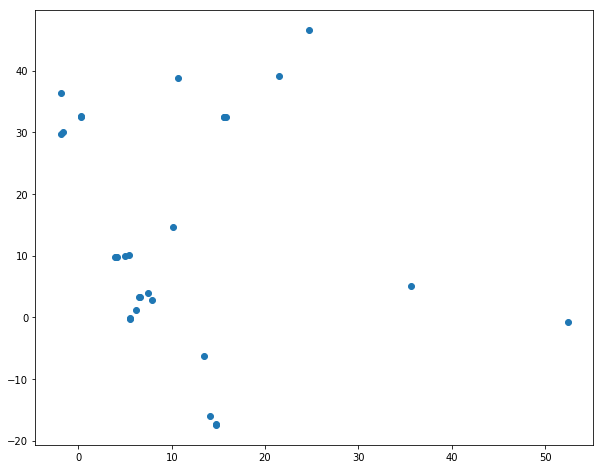
\includegraphics[scale=0.7]{1.png}
		\caption{visualizing our data set}	     
	\end{figure}
\end{center}

The next task that we perform is to normalize our data set, So we will reduce by the mean and subtract by the standard deviation in order to have numerical stability.
We obtain the following graph :

\begin{center}
	\begin{figure}
		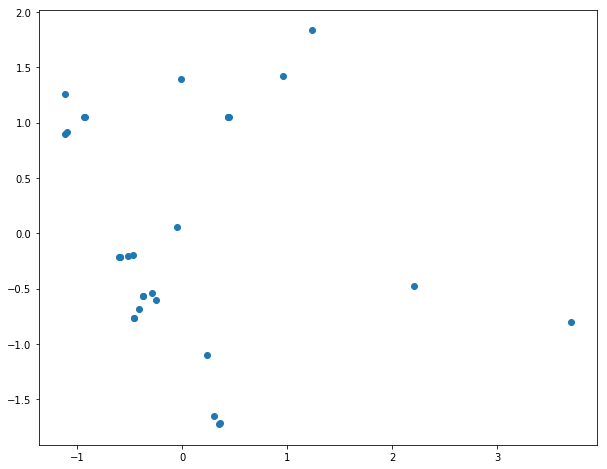
\includegraphics[scale=0.7]{2.png}
		\caption{normalized Data set}	     
	\end{figure}
\end{center}

We create a function that help us visualize the locations and shapes of the Gaussian Mixture Model clusters by drawing ellipses based on the Gaussian Mixture Model output:

The first one we consider 2 clusters :
\begin{center}
	\begin{figure}
		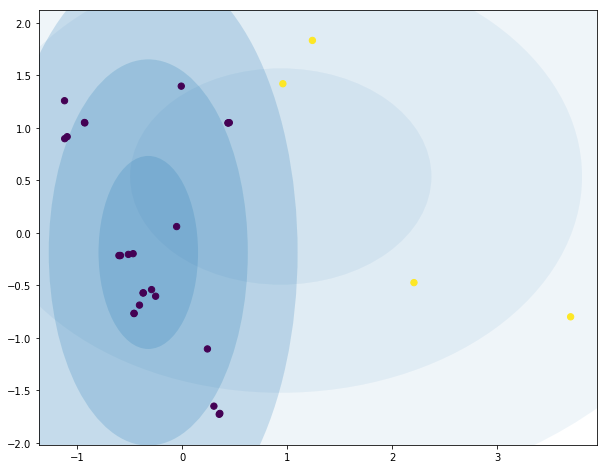
\includegraphics[scale=0.7]{4.png}
		\caption{Ellipses based on the 2 Gaussian Mixture Model output}	     
	\end{figure}
\end{center}

The second one we consider 3 clusters :
\begin{center}
	\begin{figure}
		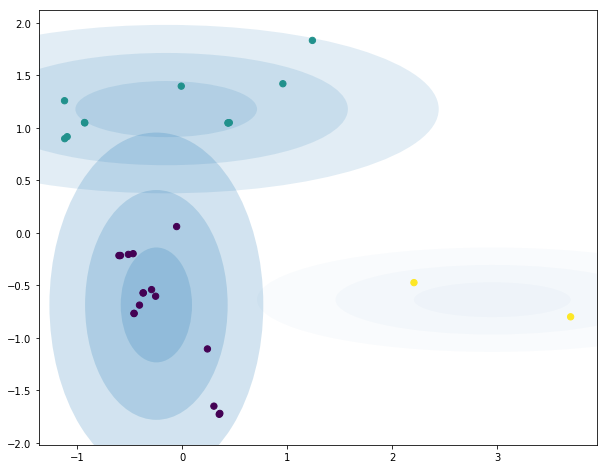
\includegraphics[scale=0.7]{3.png}
		\caption{Ellipses based on the 3 Gaussian Mixture Model output}	     
	\end{figure}
\end{center}

The third one we consider 4 clusters :
\begin{center}
	\begin{figure}
		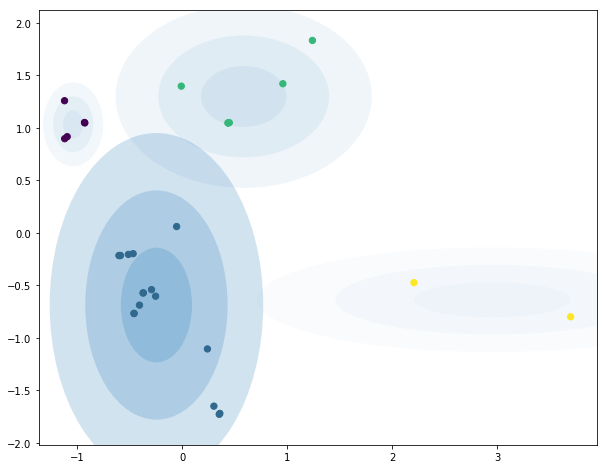
\includegraphics[scale=0.7]{5.png}
		\caption{Ellipses based on the 4 Gaussian Mixture Model output}	     
	\end{figure}
\end{center}

We take the same data and transform it, we recognize that these transformed clusters are non-circular, and thus circular clusters would be a poor fit.

we can use the Gaussian Mixture Model approach to fit our stretched dataset; allowing for a full covariance the model will fit even very oblong, stretched-out clusters:

The first one we consider 3 clusters :
\begin{center}
	\begin{figure}
		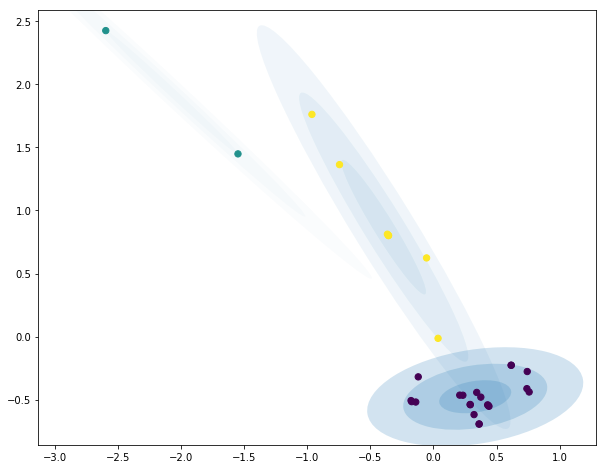
\includegraphics[scale=0.7]{6.png}
		\caption{Ellipses based on the 3 Gaussian Mixture Model output where we apply the transformation}	     
	\end{figure}
\end{center}

The second one we consider 4 clusters :
\begin{center}
	\begin{figure}
		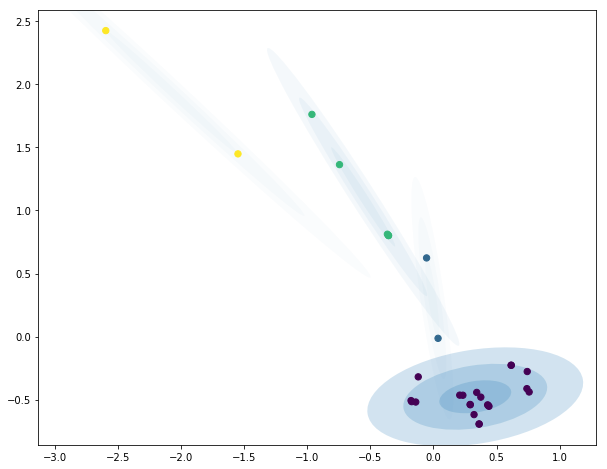
\includegraphics[scale=0.7]{7.png}
		\caption{Ellipses based on the 4 Gaussian Mixture Model output where we apply the transformation}	     
	\end{figure}
\end{center}

We can see  in the graph that if we consider just 2 mixture model , we have collision with the two ellipses but a good value for $k = 3$ from this value we can see that the ellipses are well drawn. Also for $k = 4$ it's perform very well and this can be view as over-fitting. 
\end{document}
